%!TEX root = IAL.tex

\chapter{Sistemas Lineares}

Ao longo de todo esse capítulo o conjunto $\cp{K}$ será considerado como sendo um dos conjuntos: $\rac$, $\real$ ou $\complex$.

\section{Sistemas Lineares}\label{ssub:sistemas_lineares}
Vamos trabalhar com \textbf{equações lineares}\index{Sistemas Lineares!Equação linear} em $n$ variáveis $x_1$, $x_2$, \dots, $x_n$ que são equações que podem ser escritas na forma
\begin{equation}\label{equacao_linear}
    a_1x_1  + a_2x_2 +  \cdots + a_qx_q  = b,
\end{equation}
onde $a_1$, $a_2$, \dots, $a_q$, $b$ são escalares no corpo $\cp{K}$, sendo que nem todos os coeficientes $a_i$ são nulos.

No caso em que $b = 0$,  a equação \eqref{equacao_linear} tem a forma
\begin{equation}
    a_1x_1 + a_2x_2 + \cdots + a_qx_q = 0
\end{equation}
e é chamada de uma \textbf{equação linear homogênea}\index{Sistemas Lineares!Equação linear homogênea}.

\begin{exemplos}
	\begin{enumerate}[label={\arabic*})]
		\item Equações da forma
			\begin{enumerate}
				\item $x_1 + 2x_2 - 3x_3 = 10$, em $\cp{K} = \rac$
				\item $2x_1 + 0x_2 + \sqrt{2}x_3 - 4x_4 = 0$, em $\cp{K} = \real$, que será escrita como $2x_1 + 0x_2 + \sqrt{2}x_3 - 4x_4 = 0$
				\item $ix_1 + (2 +i)x_2 = 3 + 2i$, em $\cp{K} = \complex$
			\end{enumerate}
		são exemplos de \textbf{equações lineares}.

		\item Já equações na forma
			\begin{enumerate}
				\item $x_1^2 + 2x_2 - 3x_3 = 0$ em $\cp{K} = \real$
				\item $x_1 + 2\sin(x_2) + 3x_3 + x_ 4 = 1$ em $\cp{K} = \real$
				\item $2x_1 + 3x_2 - 4x_3^{-1} = 2$ em $\cp{K} = \rac$
			\end{enumerate}
		não são equações lineares e portanto não serão abordadas nesse curso.
	\end{enumerate}
\end{exemplos}

Considerenado $\cp{K} = \real$, queremos analisar um conjuto de equações lineares do tipo:

\begin{align}
    \begin{cases}\label{sistema_linear_2x2}
        ax + by = b_1\\
        cx + dy = b_2
    \end{cases}
\end{align}
onde $a$, $b$, $c$, $d$, $b_1$, $b_2 \in \cp{K}$.

Queremos saber se é possível encontrar valores para $x$, $y$ no conjunto $\real$ de modo que essas duas equações sejam simultaneamente verdadeiras? Caso existam, gostaríamos de determinar todos os possíveis valores que $x$ e $y$ podem assumir.

Observe que cada equação linear em \eqref{sistema_linear_2x2} representa uma reta no plano cartesiano. Assim queremos determinar se essas restas possuem alguma interseção.

Mas sabemos que duas retas no plano podem ser coincidentes, paralelas ou se interceptam em um único ponto.

Assim se as retas do sistema \eqref{sistema_linear_2x2} são \textbf{coincidentes}, existem infinitos valores de $x$, $y \in \cp{K}$ que satisfazem as duas equações simultanemente. Neste caso dizemos que o sistema \eqref{sistema_linear_2x2} é \textbf{possível e indeterminado}.

\definecolor{qqqqff}{rgb}{0,0,1}
\definecolor{ffqqqq}{rgb}{1,0,0}
\begin{center}
    \begin{tikzpicture}[line cap=round,line join=round,>=triangle 45,x=1cm,y=1cm]
        \begin{axis}[
            x=1cm,y=1cm,
            axis lines=middle,
            xticklabels={,,},
            yticklabels={,,},
            xlabel=$x$,
            ylabel=$y$,
            xmin=-2,
            xmax=5,
            ymin=-1.3,
            ymax=3,]
            \draw [line width=5.2pt,dash pattern=on 1pt off 1pt,color=ffqqqq,domain=-1.348257839721257:5.807994044102577] plot(\x,{(--4-1*\x)/2});
            \draw [line width=2pt,color=qqqqff,domain=-1.348257839721257:5.807994044102577] plot(\x,{(--8-2*\x)/4});
            \begin{scriptsize}
                \draw[color=ffqqqq] (1.8,2) node {$a_{11}x + a_{12}y = b_1$};
                \draw[color=qqqqff] (3,1.5) node {$a_{21}x + a_{22}y = b_2$};
            \end{scriptsize}
        \end{axis}
    \end{tikzpicture}
\end{center}

Agora se as retas em \eqref{sistema_linear_2x2} são \textbf{paralelas}, não existem valores de $x$, $y \in \cp{K}$ satisfazendo as duas equações simultaneamente. Nesse caso dizemos que o sistema \eqref{sistema_linear_2x2} é \textbf{impossível}.

\definecolor{ffqqqq}{rgb}{1,0,0}
\definecolor{qqqqff}{rgb}{0,0,1}
\begin{center}
    \begin{tikzpicture}[line cap=round,line join=round,>=triangle 45,x=1cm,y=1cm]
        \begin{axis}[
            x=1cm,y=1cm,
            axis lines=middle,
            xticklabels={,,},
            yticklabels={,,},
            xlabel=$x$,
            ylabel=$y$,
            xmin=-5.3,
            xmax=6.3,
            ymin=-1,
            ymax=4.3,]
            \draw [line width=2pt,color=qqqqff,domain=-5:6] plot(\x,{(--4-1*\x)/5});
            \draw [line width=2pt,color=ffqqqq,domain=-5:6] plot(\x,{(--16-1*\x)/5});
            \begin{scriptsize}
                \draw[color=qqqqff] (-3.8,2.2) node {$a_{21}x + a_{22}y = b_2$};
                \draw[color=ffqqqq] (-3.8,3.4) node {$a_{11}x + a_{12}y = b_1$};
            \end{scriptsize}
        \end{axis}
    \end{tikzpicture}
\end{center}

Por fim, as retas em \eqref{sistema_linear_2x2} podem se \textbf{interceptar}. Nesse caso existe um único conjunto de valores $x = \alpha \in \cp{K}$ e $y = \lambda \in \cp{K}$ que satisfaz as duas equações simultaneamente. Neste caso dizemos que o sistema \eqref{sistema_linear_2x2} é \textbf{possível e determinado}.

\definecolor{qqqqff}{rgb}{0,0,1}
\definecolor{ffqqqq}{rgb}{1,0,0}
\begin{center}
    \begin{tikzpicture}[line cap=round,line join=round,>=triangle 45,x=1cm,y=1cm]
        \begin{axis}[
            x=1cm,y=1cm,
            axis lines=middle,
            xticklabels={,,},
            yticklabels={,,},
            xlabel=$x$,
            ylabel=$y$,
            xmin=-2,
            xmax=4.3,
            ymin=-2,
            ymax=3.5,]
            \draw [line width=2pt,color=ffqqqq,domain=-4:5] plot(\x,{(--4.94--7.92*\x)/7.58});
            \draw [line width=2pt,color=qqqqff,domain=-4:5] plot(\x,{(--4.824-8.66*\x)/8.24});
            \begin{scriptsize}
                \draw[color=ffqqqq] (2.9,2) node {$a_{11}x + a_{12}y = b_1$};
                \draw[color=qqqqff] (2.7,-0.5) node {$a_{21}x + a_{22}y = b_2$};
            \end{scriptsize}
        \end{axis}
    \end{tikzpicture}
\end{center}

Esse mesmo tipo de análise pode ser aplicada num sistema da forma
\begin{align}
    \begin{cases}\label{sistema_linear_3x3}
        a_1x + a_2y + a_3z = b_1\\
        a_4x + a_5y + a_6z = b_2\\
        a_7x + a_8y + a_9z = b_3
    \end{cases}
\end{align}
onde $a_i \in \cp{K}$ para $1 \le i \le 9$ e $b_j \in \cp{K}$ para $1 \le j \le 3$.

Neste caso as equações desse sistema representam planos no espaço tridimensional. Nesse sistema então queremos saber quais são as possíveis interseções entre estes três planos.

Temos então as seguintes possibilidades:

\begin{enumerate}
    \item Os três planos se interceptam em um único ponto. Assim existe um único conjunto de valores $x = \alpha \in \cp{K}$, $y = \lambda \in \cp{K}$ e $z = \gamma \in \cp{K}$  que satisfaz as três equações simultaneamente.  Neste caso dizemos que o sistema \eqref{sistema_linear_3x3}  é \textbf{possível e determinado}.
        \begin{figure}[h]
            \centering
            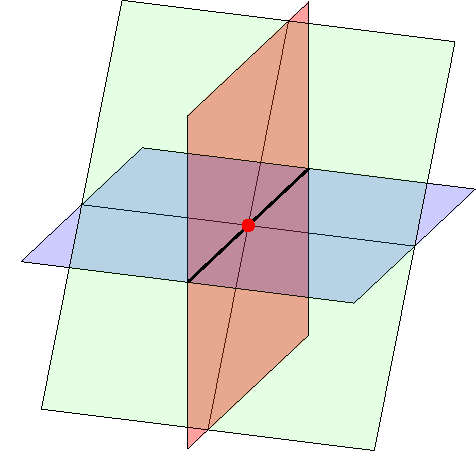
\includegraphics[scale=0.6]{3-planos-solucao-unica.pdf}
                \caption{Solução única}
        \end{figure}
    \item Os três planos se interceptam em infinitos pontos. Existem infinitos valores de $x$, $y$, $z \in \cp{K}$ que satisfazem as três equações simultanemente. Neste caso dizemos que o sistema \eqref{sistema_linear_3x3} é \textbf{possível e indeterminado}.
        \begin{figure}[h]
            \centering
            \begin{subfigure}{.32\textwidth}
                \centering
                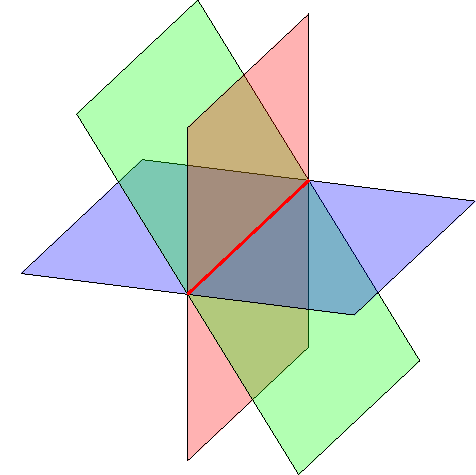
\includegraphics[width=\linewidth]{2-planos-coincidentes-infinitas-solucoes-intersecao-reta.pdf}
                \caption{Infinitas soluções}
            \end{subfigure}
            \begin{subfigure}{.32\textwidth}
                \centering
                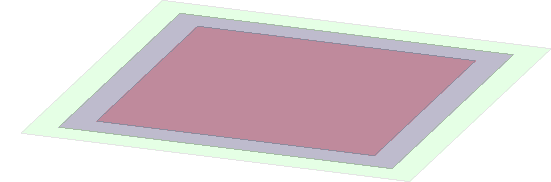
\includegraphics[width=\linewidth]{3-planos-coincidentes-infinitas-solucoes.pdf}
                \caption{Infinitas soluções}
            \end{subfigure}
            \begin{subfigure}{.32\textwidth}
                \centering
                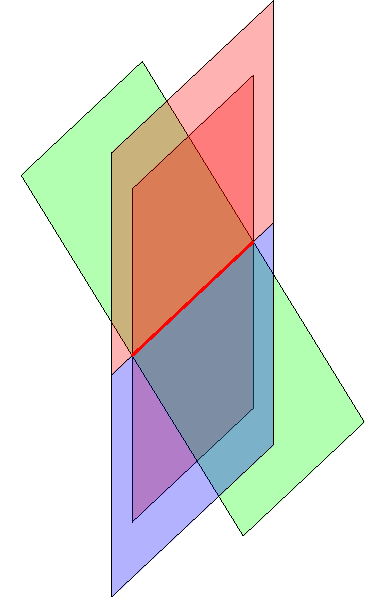
\includegraphics[width=\linewidth]{2-planos-coincidentes-terceiro-fora-infinitas-solucoes-intersecao-reta.pdf}
                \caption{Infinitas soluções}
            \end{subfigure}
        \end{figure}
    \item Os três planos não possuem uma interseção em comum. Neste caso não existem valores de $x$, $y$, $z \in \cp{K}$  satisfazendo as três equações simultaneamente. Assim dizemos que o sistema \eqref{sistema_linear_3x3}  é \textbf{impossível}.
        \begin{figure}[h]
            \centering
            \begin{subfigure}{.32\textwidth}
                \centering
                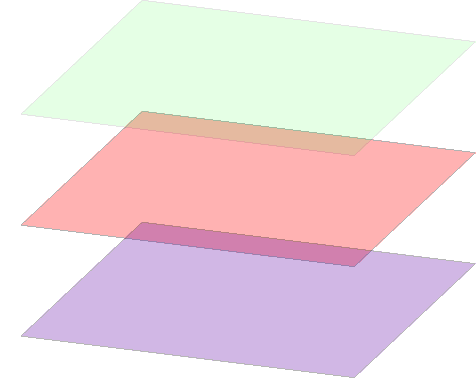
\includegraphics[width=\linewidth]{3-planos-paralelos-nenhuma-solucao.pdf}
                \caption{Nenhuma solução}
		    \end{subfigure}
            \begin{subfigure}{.32\textwidth}
                \centering
                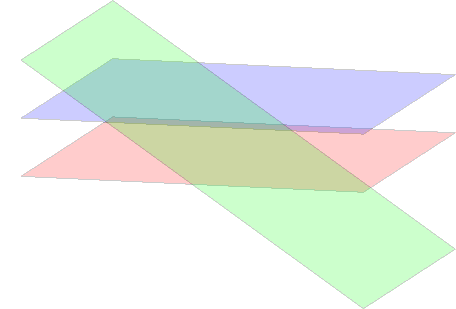
\includegraphics[width=\linewidth]{2-planos-paralelos-nenhuma-solucao.pdf}
                 \caption{Nenhuma solução}
              \end{subfigure}
            \begin{subfigure}{.32\textwidth}
                \centering  
		   
\includegraphics[width=\linewidth]{3-planos-sem-nenhuma-intersecao-dois-a-dois-retas-nenhuma-solucao.pdf}
		    \caption{Nenhuma solução}
	       \end{subfigure}
        \end{figure}
\end{enumerate}

Agora, de modo geral queremos trabalhar com uma quantidade qualquer de equações. Para isso começamos escolhendo escalares $b_1$, \dots, $b_m$  e $a_{ij}$,  $1 \le i \le m$, $1 \le j \le n$ todos em $\cp{K}$.

Queremos saber se é possível encontrar valores para  $x_1$, $x_2$, \dots, $x_n$  de modo que o seguinte conjunto de equações sejam válidas: 
\begin{equation}\label{sistema_linear_geral}
\begin{cases}
        a_{11}x_1 + a_{12}x_2 + \cdots + a_{1n}x_n = b_1\\
        a_{21}x_1 + a_{22}x_2 + \cdots + a_{2n}x_n = b_2\\
        \qquad \vdots\\
        a_{m1}x_1 + a_{m2}x_2 + \cdots + a_{mn}x_n = b_m
    \end{cases}
\end{equation}

O conjunto de equações em \eqref{sistema_linear_geral} é chamado de um  \textbf{sistema de $m$ equa\c{c}\~oes lineares  a $n$ inc\'ognitas}\index{Sistema Linear} $x_1$, $x_2$, \dots, $x_n$ , ou simplesmente de um \textbf{sistema linear}, nas incógnitas  $x_1$, $x_2$, \dots, $x_n$.

Uma solução de um sistema linear do tipo \eqref{sistema_linear_geral}
\[
    x_1 = \alpha_1,  x_2 = \alpha_2,  \dots, x_n = \alpha_n
\]
onde $\alpha_1$, $\alpha_2$, \dots, $\alpha_n \in \cp{K}$,  pode ser escrita como
\[
    (\alpha_1, \alpha_2, \dots, \alpha_n)
\]
e é chamada de uma \textbf{ênupla ordenada}\index{Sistemas linears!ênupla ordenada} ou uma \textbf{n-upla ordenada}.


Se $b_1 = b_2 = \cdots = b_m = 0_\cp{K} \in K$,  dizemos que o sistema
\begin{equation}\label{sistemalinearhomogeneo}\index{Sistema Linear}
    \begin{cases}
        a_{11}x_1 + a_{12}x_2 + \cdots + a_{1n}x_n = 0_\cp{K}\\
        a_{21}x_1 + a_{22}x_2 + \cdots + a_{2n}x_n = 0_\cp{K}\\
        \qquad \vdots\\
        a_{m1}x_1 + a_{m2}x_2 + \cdots + a_{mn}x_n = 0_\cp{K}
    \end{cases}
\end{equation}
\'e um \textbf{sistema linear homog\^eneo}.\index{Sistema linear!homogêneo} 

Observe que tal sistema sempre possui solu\c{c}\~ao,  a saber, $x_1 = x_2 = \cdots = x_n = 0_\cp{K}$.

Para o caso de sistemas lineares temos o seguinte resultado:

\begin{teorema}
    Todo sistema linear do tipo \eqref{sistema_linear_geral} tem zero,  uma  ou uma infinidade de soluções.  Não existem outras possibilidades.
\end{teorema}

No caso de um sistema linear da forma \eqref{sistema_linear_geral},  o processo para encontrar suas soluções ser\'a feito mediante o uso de 3 tipos de opera\c{c}\~oes.  S\~ao elas:
\begin{itemize}
\item[$e_1$)] Troca da posi\c{c}\~ao de duas equa\c{c}\~oes.
\item[$e_2$)] Multiplica\c{c}\~ao de uma equa\c{c}\~ao por um escalar n\~ao nulo.
\item[$e_3$)] Substitui\c{c}\~ao de uma equa\c{c}\~ao pela soma desta equa\c{c}\~ao com alguma outra.
\end{itemize}

Estas tr\^es opera\c{c}\~oes s\~ao chamadas de  \textbf{opera\c{c}\~oes elementares}.

\begin{exemplos}
	Utilizando somente operações elementares encontre as soluções dos seguintes sistemas lineares:
	\begin{enumerate}[label={\arabic*})]
		\item $\begin{cases}x + y = 4\\3x + 3y = 6\end{cases}$

		\item $\begin{cases}x + y + 2z = 9\\ 2x + 4y - 3z = 1\\ 3x + 6y - 3z = 0\end{cases}$
	\end{enumerate}

	\begin{solucao}
		\begin{enumerate}[label={\arabic*})]
			\item Neste caso podemos somar a segunda equação do sistema com ela mesma mais -3 vezes a primeira equação:
				\[
					\begin{cases}
						x + y = 4\\
						3x + 3y + (-3x) + (-3y) = 4 + (-3)\cdot 4
					\end{cases}
				\]
			que resulta em
			\[
				\begin{cases}
					x + y = 4\\
					0 = -6
				\end{cases}
			\]
			e a segunda equação desse sistema é uma contradição. Logo não existem valores para $x$ e $y$ em $\real$ que satisfazem as duas equações desse sistema simultaneamente. Portanto tal sistema é um \textbf{sistema impossível}.
                    \item Denote as linhas desse sistema por $L_1$, $L_2$ e $L_3$. Começamos trocando a linha 2, $L_2$, por ela mesma somanda com -2 vezes a linha 1, $L_1$. Denotemos essa operação por $L_2 \to L_2 - 2L_1$. Com essa operação obtemos o sistema
                        \[
                            \begin{cases}
                                x + y + 2z = 9\\
                                2y - 7z = -17\\
                                3x + 6y - 3z = 0
                            \end{cases}
                        \]
                        Agora trocamos a linha 3 por ela mesma menos 3 vezes a linha 1 ($L_3 \to L_3 - 3L_1$). Após essa operação o sistema anterior torna-se
                        \[
                            \begin{cases}
                                x + y + 2z = 9\\
                                2y - 7z = -17\\
                                3y - 9z = -27
                            \end{cases}
                        \]
                        Multiplicando a segunda linha por 1/2 ($L_2 \to \frac{1}{2}L_2$) obtemos:
                        \[
                            \begin{cases}
                                x + y + 2z = 9\\
                                y - (7/2)z = -17/2\\
                                3y - 9z = -27
                            \end{cases}
                        \]
                        Agora vamos multiplicar a segunda linha por -3 e somar com a terceira linha ($L_3 \to L_3 - 3L_2$).
                        \[
                            \begin{cases}
                                x + y + 2z = 9\\
                                y - (7/2)z = -17/2\\
                                3/2z = -3/2
                            \end{cases}
                        \]
                        Podemos multiplicar a terceira linha por 2/3 ($L_3 \to \dfrac{2}{3}L_3$) para obter:
                        \[
                            \begin{cases}
                                x + y + 2z = 9\\
                                y - (7/2)z = -17/2\\
                                z = -1
                            \end{cases}
                        \]
                        Troque a primeira linha por ela mesma menos a segunda linha ($L_1 \to L_1 - L_2$):
                        \[
                            \begin{cases}
                                x + (11/2)z = 35/2\\
                                y - (7/2)z = -17/2\\
                                z = -1
                            \end{cases}
                        \]
                        Agora trocamos a segunda linha por ela mesma mais 7/2 vezes a terceira linha ($L_2 \to L_2 + (7/2)L_3$):
                        \[
                            \begin{cases}
                                x + (11/2)z = 35/2\\
                                y  = -12\\
                                z = -1
                            \end{cases}
                        \]
                        Finalmente, trocando a primeira linha por ela mesma menos (11/2) vezes a terceira linha ($L_1 \to L_1 - (11/2)L_3$) obtemos
                        \[
                            \begin{cases}
                                x = 23\\
                                y = -12\\
                                z = -1
                            \end{cases}
                        \]
                        Assim vemos que o sistema tem uma única solução que é $x = 23$, $y = -12$ e $z = -1$.
		\end{enumerate}
	\end{solucao}
\end{exemplos}

Observe nos exemplos anteriores que a aplicação das operações elementares afeta somente os coeficientes das variáveis e os termos independentes. As variáveis do sistema permanecem inalteradas durante todo o processo. Assim não precisamos ficar repetindo as variáveis o tempo todo. Podemos tratar somente com seus coeficientes e os termos independetes do sistema.

A partir dessa observação, podemos associar ao sistema \eqref{sistema_linear_geral} uma matriz contendo os coeficientes de cada equação junto com seus respectivos termos independentes. Obtemos assim a matriz
\[
\begin{bmatrix}
        a_{11} & a_{12} & \cdots & a_{1n} & b_1\\
a_{21} & a_{22} & \cdots & a_{2n} & b_2\\
\vdots & \vdots & \vdots & \vdots & \vdots\\
a_{m1} & a_{m2} & \cdots & a_{mn} & b_m\\
    \end{bmatrix}
\]

que \'e chamada de \textbf{matriz ampliada do sistema}  ou \textbf{matriz aumentada do sistema}.

Para destacar que a última coluna dessa matriz contém os termos independentes do sistema podemos também escrever:
\[
    \begin{amatrix}{4}
        a_{11} & a_{12} & \cdots & a_{1n} & b_1\\
	a_{21} & a_{22} & \cdots & a_{2n} & b_2\\
	\vdots & \vdots & \vdots & \vdots & \vdots\\
	a_{m1} & a_{m2} & \cdots & a_{mn} & b_m\\
    \end{amatrix}
\]

\begin{exemplos}
    Escreva a matriz ampliada dos seguintes sistemas lineares:
    \begin{enumerate}[label={\arabic*})]
        \item \[\begin{cases} x_1 + x_2 - 3x_3 + x_4 = -1\\ 2x_1 - 3x_2 + x_4 = 0\\ 3x_1 + 2x_3 = -3\\ x_1 + x_4 = -2\end{cases}\]
        \item \[\begin{cases} x_1 + x_2 - 3x_3 + x_4 = -2\\ 2x_1 - 3x_2 + x_4 = 0\end{cases}\]
        \item \[\begin{cases} 2x_1 - 5x_2 + 4x_3 - 7x_4 + 8x_5 = 0\\ 3x_1 - 7x_2 + 2x_4 - 9x_5 = 0\\ 5x_3 + 8x_4 = 0\\ x_3 - x_4 = 0\end{cases}\]
    \end{enumerate}
    \begin{solucao}
        \begin{enumerate}[label={\arabic*})]
            \item Neste caso a matriz ampliada é:
                \[
                    \begin{amatrix}{4}
                        1 & 1 & -3 & 1 & -1\\
                        2 & -3 & 0 & 1 & 0\\
                        3 & 0 & 2 & 0 & -3\\
                        1 & 0 & 0 & 1 & -2
                    \end{amatrix}
                \]
            \item Neste caso a matriz ampliada é:
                \[
                    \begin{amatrix}{4}
                        1 & 1 & -3 & 1 & -2\\
                        2 & -3 & 0 & 1 & 0\\
                    \end{amatrix}
                \]
            \item Neste caso a matriz ampliada é:
                \[
                    \begin{amatrix}{5}
                        2 & -5 & 4 & -7 & 8 & 0\\
                        3 & -7 & 0 & 2 & -9 & 0\\
                        0 & 0 & 5 & 8 & 0 & 0\\
                        0 & 0 & 1 & -1 & 0 & 0
                    \end{amatrix}
                \]
                Como a última coluna dessa matriz é composta somente de zeros podemos omití-la e escrever:
                \[
                    \begin{bmatrix}
                        2 & -5 & 4 & -7 & 8\\
                        3 & -7 & 0 & 2 & -9\\
                        0 & 0 & 5 & 8 & 0\\
                        0 & 0 & 1 & -1 & 0 
                    \end{bmatrix}
                \]

        \end{enumerate}
    \end{solucao}
\end{exemplos}
Na forma matricial as opera\c{c}\~oes elementares s\~ao descritas como:

\vspace{.3cm}

\begin{itemize}
    \item[$e_1$)] Trocar a $i$-\'esima linha de $A$ pela $j$-\'esima linha de $A$: $L_i \leftrightarrow L_j$;

    \item[$e_2$)] Multiplica\c{c}\~ao da $i$-\'esima linha de $A$ por um escalar $\alpha \in \cp{K}$ n\~ao nulo: $L_i \rightarrow \alpha L_i$;

   \item[$e_3$)] Substitui\c{c}\~ao da $i$-\'esima linha de $A$ pela $i$-\'esima linha mais $\alpha$ vezes a $j$-\'esima linha: $L_i \rightarrow L_i + \alpha L_j$.
\end{itemize}

O que iremos fazer para resolver um sistema linear do tipo \eqref{sistema_linear_geral} é aplicar operações operações elementares na linhas da matriz ampliada até que ela esteja num formato especial. Esse formato que buscamos é o seguinte:

\begin{definicao}\label{linhareduzida}
    Uma matriz $A$ $m \times n$ \'e  dita estar na \textbf{forma escalonada reduzida por linhas} se:
    \begin{enumerate}[label={\roman*})]
        \item O primeiro elemento n\~ao nulo em cada linha n\~ao nula de $A$ \'e $1$. Dizemos que esse número 1 é um \textbf{pivô}.

        \item Toda linha de $A$ cujos elementos s\~ao todos nulos ocorre abaixo de todas as linhas que possuem um elemento n\~ao-nulo. 

        \item Se as linhas 1, 2, \dots, $r$ s\~ao as linhas n\~ao-nulas de $A$ e se o \textbf{pivô} da linha $i$ ocorre na coluna $k_i$, $i = 1$, \dots, $r$, ent\~ao $k_1 < k_2 < \cdots < k_r$.

        \item Cada coluna de $A$ que cont\'em um \textbf{pivô} tem todos os seus outros elementos nulos.
    \end{enumerate}
\end{definicao}

\begin{observacao}
    Uma matriz que satisfaz as três primeiras propriedades da definição anterior é dita estar na \textbf{forma escalonada por linhas}, ou simplesmente, em \textbf{forma escalonada}.
\end{observacao}

\begin{exemplos}
    \begin{enumerate}[label={\arabic*})]
        \item As seguintes matrizes estão na \textbf{forma escalonada reduzida por linhas}:
            \begin{align*}
                \begin{bmatrix}
                    1 & 0 & 0 & 4\\
                    0 & 1 & 0 & 7\\
                    0 & 0 & 1 & 1
                \end{bmatrix};
                \begin{bmatrix}
                    0 & 1 & i & 3 & 3\\
                    0 & 0 & 0 & 1 & -2 + 4i\\
                    0 & 0 & 0 & 0 & 0
                \end{bmatrix};
                \begin{bmatrix}
                    0 & 0\\
                    0 & 0
                \end{bmatrix};
                \begin{bmatrix}
                    1 & 0 & 0\\
                    0 & 1 & 0\\
                    0 & 0 & 1
                \end{bmatrix}.
            \end{align*}

        \item Já as seguintes matrizes estão na \textbf{forma escalonada}:
            \begin{align*}
                \begin{bmatrix}
                    1 & 4 & -3 & 7\\
                    0 & 1 & 6 & 2\\
                    0 & 0 & 1 & 5
                \end{bmatrix};
                \begin{bmatrix}
                    1 & 1 & 0\\
                    0 & 1 & 0\\
                    0 & 0 & 0
                \end{bmatrix};
                \begin{bmatrix}
                    0 & 1 & 2 & 3 & 0\\
                    0 & 0 & 0 & 1 & 1\\
                    0 & 0 & 0 & 0 & 1
                \end{bmatrix}.
            \end{align*}
        \item Usando a matriz ampliada e as operações elementares sobre as linhas da matriz resolva o seguinte sistema:
            \[
                \begin{cases}
                    2x_1 - 4x_2 - x_3 = 1\\
                    x_1 - 3x_2 + x_3 = 1\\
                    3x_1 - 5x_2 - 3x_3 = 1
                \end{cases}
            \]
            \begin{solucao}
                Começamos montando a matriz ampliada do sistema:
                \[
                    \begin{amatrix}{3}
            		2 & -4 & -1 & 1\\
        		1 & -3 & 1 & 1\\
		        3 & -5 & -3 & 1
                    \end{amatrix}.
                \]
                Vamos aplicar as operações elementares nessa matriz:
                \begin{align*}
                    &\begin{bmatrix}
                        2 & -4 & -1 & 1\\
        		1 & -3 & 1 & 1\\
		        3 & -5 & -3 & 1
                    \end{bmatrix}
                    \begin{array}{l}
                        L_1 \leftrightarrow L_2\\\phantom{x} \\\phantom{x} 
                    \end{array} \sim
                    \begin{bmatrix}
        		1 & -3 & 1 & 1\\
                        2 & -4 & -1 & 1\\
		        3 & -5 & -3 & 1
                    \end{bmatrix}
                    \begin{array}{l}
                        \phantom{x}\\  L_2 \to L_2 - 2L_1\\\phantom{x}
                    \end{array} \sim\\
                    &\begin{bmatrix}
        		1 & -3 & 1 & 1\\
                        0 & 2 & -3 & -1\\
		        3 & -5 & -3 & 1
                    \end{bmatrix}
                    \begin{array}{l}
                        \phantom{x}\\ \phantom{x}\\ L_3 \to L_3 - 3L_1
                    \end{array} \sim
                    \begin{bmatrix}
        		1 & -3 & 1 & 1\\
                        0 & 2 & -3 & -1\\
		        0 & 4 & -6 & -2
                    \end{bmatrix}
                    \begin{array}{l}
                        \phantom{x}\\ \phantom{x}\\ L_3 \to L_3 - 2L_1
                    \end{array} \sim\\
                    &\begin{bmatrix}
        		1 & -3 & 1 & 1\\
                        0 & 2 & -3 & -1\\
		        0 & 0 & 0 & 0
                    \end{bmatrix}
                    \begin{array}{l}
                        \phantom{x}\\ L_2 \to \dfrac{1}{2}L_2\\\phantom{x}
                    \end{array} \sim
                    \begin{bmatrix}
        		1 & -3 & 1 & 1\\
                        0 & 1 & -3/2 & -1/2\\
		        0 & 0 & 0 & 0
                    \end{bmatrix}
                    \begin{array}{l}
                        L_1 \to L_1 + 3L_2\\\phantom{x}\\\phantom{x}
                    \end{array} \sim\\
                    &\begin{bmatrix}
        		1 & 0 & -7/2 & -1/2\\
                        0 & 1 & -3/2 & -1/2\\
		        0 & 0 & 0 & 0
                    \end{bmatrix}
                \end{align*}
                Essa última matriz está na forma escalonada reduzida por linhas. Assim obtemos o sistema
                \[
                    \begin{cases}
                        x_1 - (7/2)x_3 = -1/2\\
                        x_2 - (3/2)x_3 = -1/2
                    \end{cases}.
                \]

                Desse sistema obtemos
                \[
                    x_2 = -\dfrac{1}{2} + \dfrac{3}{2}x_3
                \]
                e substituindo essa equação na primeira encontramos
                \[
                    x_1 = -\dfrac{1}{2} + \dfrac{7}{2}x_3.
                \]
                Portanto fazendo $x_3 = t \in \real$ a solução desse sistema pode ser escrita como
                \[
                    x_1 = -\dfrac{1}{2} + \dfrac{7}{2}t, x_2 = -\dfrac{1}{2} + \dfrac{3}{2}t, x_3 = t, t \in \real.
                \]
                Logo o sistema é possível e indeterminado.
            \end{solucao}
    \end{enumerate}
\end{exemplos}
    
\begin{definicao}
    Se $A$ e $B$ s\~ao matrizes $m \times n$, dizemos que $B$ \'e \textbf{linha-equivalente}\index{Matrizes!linha-equivalente} a $A$, se $B$ for obtida de $A$ atrav\'es de uma quantidade finita de opera\c{c}\~oes elementares sobre as linhas de $A$.
\end{definicao}

\begin{notacao}
    $A \rightarrow B$ ou $A \sim B$.
\end{notacao}

\begin{exemplos}
    \begin{enumerate}[label={\arabic*})]
        \item As matrizes
            \[
                A = \begin{pmatrix}
                        1 & 2 & -1 & 0\\
                        0 & 1 & 3 & 4\\
                        2 & 0 & 1 & 3
                    \end{pmatrix}
                    \mbox{ e }
                B = \begin{pmatrix}
                        0 & 1 & 3 & 4\\
                        1 & 2 & -1 & 0\\
                        2 & 0 & 1 & 3
                    \end{pmatrix}
            \]
            são matrizes linha-equivalentes pois podemos obter a matriz $B$ de $A$ trocando a primeira linha de $A$ com a segunda linha. Assim $B \sim A$.
            
            Observe que também podemos obter a matriz $A$ a partir de $B$ simplesmente trocando a primeira linha de $B$ com a segunda linha. Logo $A \sim B$.
        \item As matrizes
            \[
                C = \begin{pmatrix}
                        1 & 0 & 3 & 0\\
                        2 & 1 & 0 & 1\\
                        -1 & 3 & 2 & 1
                    \end{pmatrix}
                    \mbox{ e }
                D = \begin{pmatrix}
                        1 & 0 & 3 & 0\\
                        4 & 1 & 6 & 1\\
                        0 & 3 & 5 & 1
                    \end{pmatrix}
            \]
            também são linha-equivalentes. De fato, partindo de $C$ podemos efetuar as seguintes operações elementares:
            \begin{align*}
                C &= \begin{pmatrix}
                    1 & 0 & 3 & 0\\
                    2 & 1 & 0 & 1\\
                    -1 & 3 & 2 & 1
                \end{pmatrix}
                \begin{array}{l}
                    \phantom{x}\\ L_2 \to L_2 + 2L_1\\\phantom{x}
                \end{array} \sim
                \begin{pmatrix}
                    1 & 0 & 3 & 0\\
                    4 & 1 & 6 & 1\\
                    -1 & 3 & 2 & 1
                \end{pmatrix}
                \begin{array}{l}
                    \phantom{x}\\ \phantom{x}\\ L_3 \to L_2 + L_1
                \end{array}\\ \sim
                  &\begin{pmatrix}
                    1 & 0 & 3 & 0\\
                    4 & 1 & 6 & 1\\
                    0 & 3 & 5 & 1
                \end{pmatrix} = D
            \end{align*}
            Assim $D \sim C$.

            Poderíamos fazer o contrário, começar de $D$ e obter a matriz $C$:
            \begin{align*}
                D &= \begin{pmatrix}
                    1 & 0 & 3 & 0\\
                    4 & 1 & 6 & 1\\
                    0 & 3 & 5 & 1
                \end{pmatrix}
                \begin{array}{l}
                    \phantom{x}\\ L_2 \to L_2 - 2L_1\\\phantom{x}
                \end{array} \sim
                \begin{pmatrix}
                    1 & 0 & 3 & 0\\
                    2 & 1 & 0 & 1\\
                    0 & 3 & 5 & 1
                \end{pmatrix}
                \begin{array}{l}
                    \phantom{x}\\ \phantom{x}\\ L_3 \to L_3 - L_1
                \end{array}\\ \sim
                  &\begin{pmatrix}
                    1 & 0 & 3 & 0\\
                    2 & 1 & 0 & 1\\
                    -1 & 3 & 2 & 1
                \end{pmatrix} = C
            \end{align*}

            Assim $C \sim D$.
    \end{enumerate}
\end{exemplos}
\begin{teorema}
    Duas matrizes $A$ e $B$ são equivalentes por linha se, e somente, se elas puderem ser reduzidas à mesma forma escalonada por linhas.
\end{teorema}

\begin{teorema}
    Se as matrizes ampliadas de dois sistemas lineares são equivalentes por linhas, então os dois sistemas possuem as mesmas soluções.
\end{teorema}

O \textbf{método de eliminação de Gauss}\index{Sistemas lineares!método de eliminação de Gauss} ou \textbf{método de eleminação gaussiana}\index{Sistemas lineares!eliminação gaussiana} consiste em substituir um dado sistema de equações lineares  por outro \textbf{equivalente}, que seja mais simples de ser solucionado e que tenha a mesma solução do sistema original.

\begin{definicao}[Método de eliminaçao de Gauss]
    Seja $A$ a matriz ampliada de um sistema linear. O método de \textbf{eliminação de Gauss} consiste em:
    \begin{enumerate}[label={\roman*})]
        \item Escreva a matriz ampliada do sistema de equações lineares.

        \item Use operações elementares nas linhas de $A$ para reduzir a matriz ampliada à \textbf{forma escalonada por linhas}.
        
        \item Quando a matriz ampliada estiver na forma escalonada, usando substituição de trás para a frente, resolva o sistema equivalente que corresponde a matriz escalonada reduzida por linhas.
    \end{enumerate}
\end{definicao}

\begin{observacao}
    No momento de aplicar o passo 2 do método de eliminação de Guass, temos várias escolhas que podemos fazer. Algumas dicas para a escolha da operação são as seguintes:
    \begin{enumerate}[label=({\alph*})]
        \item Localize a coluna mais à esquerda que não é toda formada por zeros.
        
        \item Crie um \textbf{pivô} no topo desta coluna.
         
        \item Use o \textbf{pivô} para criar zeros abaixo dele.

        \item Faça a linha contendo este \textbf{pivô} ir para a parte de cima e volte ao passo (a) para repetir o procedimento com o restante da submatriz. Pare quando toda a matriz estiver na forma escalonada por linhas.
    \end{enumerate}
\end{observacao}

\begin{exemplos}
    \begin{enumerate}[label={\arabic*})]
        \item Encontre a solução do seguinte sistema em $\rac$:
        \[
            \begin{cases}
                6x_3 + 19x_5 + 11x_6 = -27\\
                3x_1 + 12x_2 + 9x_3 - 6x_4 + 26x_5 + 31x_6 = -63\\
                x_1 + 4x_2 + 3x_3 - 2x_4 + 10x_5 + 9x_6 = -17\\
                -x_1 - 4x_2 - 4x_3 + 2x_4 - 13x_5 - 11x_6 = 22
            \end{cases}
        \]
        \item Considere o seguinte sistema em $\real$:
        \[
            \begin{cases}
                2x_1 + 4x_5 = 16\\
                5x_1 - 2x_2 = 4\\
                10x_1 - 4x_2 = 3
            \end{cases}
        \]
        \item Estude o seguinte sistema linear:
        \[
            \begin{cases}
                x_1 - x_2 + kx_3 = 1\\
                2x_1 + x_2 + x_3 = 0\\
                x_1 + 2x_2 + (1 - k)x_3 = k
            \end{cases}
        \]
        onde $k \in \real$. Isto é, decida para quais valores de $k \in \real$ esse sistema admite solução única, infinitas soluções e nenhuma solução.
    \end{enumerate}
    \begin{solucao}
        \begin{enumerate}
            \item Primeiro montamos a matriz ampliada do sistema:
            \[
                \begin{amatrix}{6}
                    0 & 0 & 6 & 0 & 19 & 11 & -27\\
                    3 & 12 & 9 & -6 & 26 & 31 & -63\\
                    1 & 4 & 3 & -2 & 10 & 9 & -17\\
                    -1 & -4 & -4 & 2 & -13 & -11 & 22
                \end{amatrix}
            \]
            O primeiro passo e colocar um pivô na primeira linha. Para isso podemos trocar as linhas 1 e 3 de posição: $L_1 \leftrightarrow L_3$:
            \[
               \begin{amatrix}{6}
                    1 & 4 & 3 & -2 & 10 & 9 & -17\\
                    3 & 12 & 9 & -6 & 26 & 31 & -63\\
                    0 & 0 & 6 & 0 & 19 & 11 & -27\\
                    -1 & -4 & -4 & 2 & -13 & -11 & 22
               \end{amatrix}
            \]
            Agora vamos zerar todos os elementos na primeira coluna abaixo do 1:
            \begin{align*}
                &\begin{amatrix}{6}
                    1 & 4 & 3 & -2 & 10 & 9 & -17\\
                    3 & 12 & 9 & -6 & 26 & 31 & -63\\
                    0 & 0 & 6 & 0 & 19 & 11 & -27\\
                    -1 & -4 & -4 & 2 & -13 & -11 & 22
                \end{amatrix}
                \begin{array}{l}
                    \phantom{x}\\L_2 \to L_2 - 3L_1\\\phantom{x}\\L_4 \to L_4 + L_1
                \end{array}\sim\\
                &\begin{amatrix}{6}
                    1 & 4 & 3 & -2 & 10 & 9 & -17\\
                    0 & 0 & 0 & 0 & -4 & 4 & -12\\
                    0 & 0 & 6 & 0 & 19 & 11 & -27\\
                    0 & 0 & -1 & 0 & -3 & -2 & 5
                \end{amatrix}
            \end{align*}
            Na quarta linha temos um -1 na terceira coluna. Por isso, podemos trocar a segunda e a quarta linhas de posição: $L_2 \leftrightarrow L_4$
            \[
                \begin{amatrix}{6}
                    1 & 4 & 3 & -2 & 10 & 9 & -17\\
                    0 & 0 & -1 & 0 & -3 & -2 & 5\\
                    0 & 0 & 6 & 0 & 19 & 11 & -27\\
                    0 & 0 & 0 & 0 & -4 & 4 & -12
                \end{amatrix}
            \]
            Multiplicamos a segunda linha por -1 para obter um pivô na terceira coluna:
            \[
                \begin{amatrix}{6}
                    1 & 4 & 3 & -2 & 10 & 9 & -17\\
                    0 & 0 & 1 & 0 & 3 & 2 & -5\\
                    0 & 0 & 6 & 0 & 19 & 11 & -27\\
                    0 & 0 & 0 & 0 & -4 & 4 & -12
                \end{amatrix}
            \]
            Agora vamos zerar todos os coeficientes que estão na terceira coluna e abaixo do pivô:
            \begin{align*}
                &\begin{amatrix}{6}
                    1 & 4 & 3 & -2 & 10 & 9 & -17\\
                    0 & 0 & 1 & 0 & 3 & 2 & -5\\
                    0 & 0 & 6 & 0 & 19 & 11 & -27\\
                    0 & 0 & 0 & 0 & -4 & 4 & -12
                \end{amatrix}
                \begin{array}{l}
                    \phantom{x}\\ \phantom{x}\\ L_3 \to L_3 - 6L_2\\ \phantom{x} 
                \end{array}\sim\\
                &\begin{amatrix}{6}
                    1 & 4 & 3 & -2 & 10 & 9 & -17\\
                    0 & 0 & 1 & 0 & 3 & 2 & -5\\
                    0 & 0 & 0 & 0 & 1 & -1 & 3\\
                    0 & 0 & 0 & 0 & -4 & 4 & -12
                \end{amatrix}
            \end{align*}
            Como na terceira linha já temos um pivô na quinta coluna, vamos somente zerar os coeficientes abaixo desse pivô.
            \begin{align*}
                &\begin{amatrix}{6}
                    1 & 4 & 3 & -2 & 10 & 9 & -17\\
                    0 & 0 & 1 & 0 & 3 & 2 & -5\\
                    0 & 0 & 0 & 0 & 1 & -1 & 3\\
                    0 & 0 & 0 & 0 & -4 & 4 & -12
                \end{amatrix}
                \begin{array}{l}
                    \phantom{x}\\ \phantom{x}\\ \phantom{x}\\ L_4 \to L_4 - 4L_3 
                \end{array}\sim\\
                &\begin{amatrix}{6}
                    1 & 4 & 3 & -2 & 10 & 9 & -17\\
                    0 & 0 & 1 & 0 & 3 & 2 & -5\\
                    0 & 0 & 0 & 0 & 1 & -1 & 3\\
                    0 & 0 & 0 & 0 & 0 & 0 & 0
                \end{amatrix}
            \end{align*}
            Como essa matriz está na forma escalonada temos o seguinte sistema:
            \[
                \begin{cases}
                    x_1 + 4x_2 + 3x_3 - 2x_4 + 10x_5 + 9x_6 = -17\\
                    x_3 + 3x_5 + 2x_6 = -5\\
                    x_5 - x_6 = 3
                \end{cases}
            \]
            As variáveis $x_2$, $x_4$ e $x_6$ são chamadas de \textbf{variáveis livres} do sistema linear pois não estão associadas a nenhum \textbf{pivô} na matriz escalonada desse sistema.
            Da terceira equação temos
            \[
                x_5 = 3 + x_6.
            \]
            Substituindo esse valor na segunda equação:
            \begin{align*}
                x_3 + 3(3 + x_6) + 2x_6 = -5\\
                x_3 + 9 + 3x_6 + 2x_6 = -5\\
                x_3 = -14 - 5x_6
            \end{align*}
            Finalmente, substituindo os valores encontrados para $x_3$ e $x_5$ na primeira equação:
            \begin{align*}
                x_1 + 4x_2 + 3(-14 - 5x_6) - 2x_4 + 10(3 + x_6) + 9x_6 = -17\\
                x_1 + 4x_2 - 42 - 15x_6 - 2x_4 + 30 + 10x_6 + 9x_6 = -17\\
                x_1 = -5 - 4x_2 + 2x_4 - 4x_6
            \end{align*}

            Fazendo $x_2 = s$, $x_4 = t$ e $x_6 = z$ com $s$, $t$ e $z \in \rac$ podemos escrever
            \begin{align*}
                x_1 &= -5 - 4s + 2t - 4z\\
                x_2 &= s\\
                x_3 &= -14 - 5z\\
                x_4 &= t\\
                x_5 &= 3 + z\\
                x_6 &= z
            \end{align*}
            Nesse caso temos um sistema \textbf{possível e indeterminado}. O sistema admite infinitas soluções. Podemos escrever as soluções desse sistema como o conjunto
            \[
                S = \{(-5 - 4s + 2t - 4z, s, -14 - 5z, t, 3 + z, z) \mid s, t, z \in \rac\}
            \]
            que é chamado de \textbf{conjunto-solução} do sistema linear.

            \item A matriz ampliada do sistema é
                \[
                    \begin{amatrix}{2}
                        2 & 4 & 16\\
                        5 & 2 & 4\\
                        10 & 4 & 3
                    \end{amatrix}
                \]
                Primeiro multiplicamos a linha 1 por 1/2 para termos um pivô na primeira coluna:
                \begin{align*}
                    \begin{amatrix}{2}
                        2 & 4 & 16\\
                        5 & 2 & 4\\
                        10 & 4 & 3
                    \end{amatrix}
                    \begin{array}{l}
                        L_1 \to \dfrac{1}{2}L_1\\\phantom{x}\\\phantom{x}
                    \end{array}\sim
                    \begin{amatrix}{2}
                        1 & 2 & 8\\
                        5 & 2 & 4\\
                        10 & 4 & 3
                    \end{amatrix}
                \end{align*}
                Agora vamos zerar os demais coeficientes na primeira coluna:
                \begin{align*}
                    \begin{amatrix}{2}
                        1 & 2 & 8\\
                        5 & 2 & 4\\
                        10 & 4 & 3
                    \end{amatrix}
                    \begin{array}{l}
                        \phantom{x}\\L_2 \to L_2 - 5L_1\\L_3 \to L_3 - 10L_1
                    \end{array}\sim
                    \begin{amatrix}{2}
                        1 & 2 & 8\\
                        0 & -8 & -36\\
                        0 & -16 & -77
                    \end{amatrix}
                \end{align*}
                Agora vamos criar um pivô na segunda linha, segunda coluna. Para isso fazemos:
                \begin{align*}
                    \begin{amatrix}{2}
                        1 & 2 & 8\\
                        0 & -8 & -36\\
                        0 & -16 & -77
                    \end{amatrix}
                    \begin{array}{l}
                        \phantom{x}\\L_2 \to -\dfrac{1}{8}\\\phantom{x}
                    \end{array}\sim
                    \begin{amatrix}{2}
                        1 & 2 & 8\\
                        0 & 1 & 9/4\\
                        0 & -16 & -77
                    \end{amatrix}
                \end{align*}
                Por último podemos zerar o coeficiente abaixo do pivô da segunda linha:
                \begin{align*}
                    \begin{amatrix}{2}
                        1 & 2 & 8\\
                        0 & 1 & 9/4\\
                        0 & -16 & -77
                    \end{amatrix}
                    \begin{array}{l}
                        \phantom{x}\\\phantom{x}\\L_3 \to L_3 + 16L_2!
                    \end{array}\sim
                    \begin{amatrix}{2}
                        1 & 2 & 8\\
                        0 & 1 & 9/4\\
                        0 & 0 & -5
                    \end{amatrix}
                \end{align*}
                Dessa última matriz, obtemos o sistema
                \[
                    \begin{cases}
                        x_1 - 2x_2 = 8\\
                        x_2 = 3\\
                        0 = -5
                    \end{cases}
                \]
                A última equação desse sistema não admite solução. Logo tal sistema é impossível.
                \item A matriz ampliada desse sistema é:
                \[
                    \begin{amatrix}{3}
                        1 & -1 & k & 1\\
                        2 & 1 & 1 & 0\\
                        1 & 2 & 1 - k & k\\
                    \end{amatrix}    
                \]
                Apliquemos a eliminação gaussiana
                \begin{align*}
                    &\begin{amatrix}{3}
                        1 & -1 & k & 1\\
                        2 & 1 & 1 & 0\\
                        1 & 2 & 1 - k & k\\
                    \end{amatrix}
                    \begin{array}{l}
                        \phantom{x}\\L_2 \to L_2 - 2L_1\\L_3 \to L_3 - L_1
                    \end{array}\sim
                    \begin{amatrix}{3}
                        1 & -1 & k & 1\\
                        0 & 3 & 1 - 2k & -2\\
                        0 & 3 & 1 - 2k & k - 1\\
                    \end{amatrix}
                    \begin{array}{l}
                        \phantom{x}\\\phantom{x}\\L_3 \to L_3 - L_2
                    \end{array}\\ &\sim
                    \begin{amatrix}{3}
                        1 & -1 & k & 1\\
                        0 & 3 & 1 - 2k & -2\\
                        0 & 0 & 0 & k + 1\\
                    \end{amatrix}
                    \begin{array}{l}
                        \phantom{x}\\L_2 \to \dfrac{1}{3}L_2\\\phantom{x}
                    \end{array}\sim
                    \begin{amatrix}{3}
                        1 & -1 & k & 1\\
                        0 & 1 & (1 - 2k)/3 & -2/3\\
                        0 & 0 & 0 & k + 1\\
                    \end{amatrix}
                \end{align*}
                Da última linha dessa matriz temos que se $k + 1 \ne 0$, isto é, $k \ne -1$ então o sistema é impossível. Então para qualquer $K \in \real$ com $k \ne -1$ o sistema é impossível.

                Se $k = -1$, a última matriz torna-se
                \[
                    \begin{amatrix}{3}
                        1 & -1 & -1 & 1\\
                        0 & 1 & 1 & -2/3\\
                        0 & 0 & 0 & 0\\
                    \end{amatrix}
                \]
                Com isso obtemos as equações
                \[
                    \begin{cases}
                        x_1 = 1/3\\
                        x_2 + x_3 = -2/3
                    \end{cases}
                \]
                Da segunda equação desse sistema encontramos
                \[
                    x_2 = -\dfrac{2}{3} - x_3
                \]
                Com isso, $x_3$ é uma variável livre. Daí, quando $k = -1$ o sistema é possível e indeterminado. O conjunto-solução é
                \[
                    S = \{(1/3, -2/3 - x_3, x_3) \mid x_3 \in \real\}.
                \]
        \end{enumerate}
    \end{solucao}
\end{exemplos}

Considere o sistema linear:
\begin{equation*}
    \begin{cases}
        a_{11}x_1 + a_{12}x_2 + \cdots + a_{1n}x_n = b_1\\
        a_{21}x_1 + a_{22}x_2 + \cdots + a_{2n}x_n = b_2\\
        \qquad \vdots\\
        a_{m1}x_1 + a_{m2}x_2 + \cdots + a_{mn}x_n = b_m
    \end{cases}
\end{equation*}
A matriz
\[
    A = \begin{bmatrix}
        a_{11} & a_{12} & \cdots & a_{1n}\\
        a_{21} & a_{22} & \cdots & a_{2n}\\
        \vdots & \vdots & \cdots & \vdots\\
        a_{m1} & a_{m2} & \cdots & a_{mn}
    \end{bmatrix}
\]
é chamada de \textbf{matriz dos coeficientes} do sistema linear.

\begin{definicao}
    Seja $A$ a matriz ampliada de um sistema linear. Se $A$ está na forma escalonada reduzida por linhas, então as variáveis desse 
    sistema que não correspondem aos pivôs são chamadas de \textbf{variáveis livres}.\index{Sistemas lineares!variáveis livres}
\end{definicao}

\begin{definicao}
    O \textbf{posto}\index{Matriz!posto}, denotado $\p{A}$ ou $p(A)$, de uma matriz $A$ é número de linhas não nulas de qualquer 
    uma de suas formas escalonadas por linhas.
\end{definicao}

\begin{teorema}[Teorema do Posto]
    Seja $A$ a matriz dos coeficientes de um sistema linear com $n$ variáveis. Então
    \[
        \mbox{número de variáveis livres} =  n - \p{A}.
    \]
\end{teorema}

Durante a aplicação do \textbf{método de eliminação de Gauss}, paramos quando a matriz ampliada do sistema está na forma escalonada.
Todavia podemos continuar aplicando operações elementares até que a matriz atinja a forma escalonada reduzida por linhas. Esse é o caso do 
\textbf{método de Gaus-Jordan}.

\begin{definicao}[Método de eliminaçao de Gauss-Jordan]
    O método de \textbf{eliminação de Gauss-Jordan}, para solução de um sistema linear, consiste em:
    \begin{enumerate}[label={\roman*})]
        \item Escreva a matriz ampliada do sistema de equações lineares.

        \item Use operações elementares nas linhas de $A$ para reduzir a matriz ampliada à \textbf{forma escalonada reduzida por linhas}.
        
        \item Se o sistema resultante for possível, resolva-o para as variáveis dependentes em termos de quaisquer variáveis livres que 
            tenham sobrado.
    \end{enumerate}
\end{definicao}
\begin{exemplo}
    Resolva os seguintes sistemas usando o método de Guass-Jordan. Encontre o posto e o número de variáveis livres:
    \begin{enumerate}
        \item $\begin{cases}
                x_1 + 2x_2 - x_3 = 9\\
                2x_1 - x_2 + x_3 = 0\\
                4x_1 - x_2 + x_3 = 4
            \end{cases}$

        \item $\begin{cases}
                w + x + 2y + z = 0\\
                w - x - y + z = 0\\
                x + y = 0\\
                w + x + z = 0
        \end{cases}$
    \end{enumerate}
    \begin{solucao}
        \begin{enumerate}
            \item A matriz ampliada do sistema é
                \[
                    \begin{amatrix}{3}
                        1 & 2 & -1 & 9\\
                        2 & -1 & 1 & 0\\
                        4 & -1 & 1 & 4
                    \end{amatrix}
                \]
                Aplicando ométodo de Guass-Jordan à essa matriz:
                \begin{align*}
                &\begin{amatrix}{3}
                    1 & 2 & -1 & 9\\
                    2 & -1 & 1 & 0\\
                    4 & -1 & 1 & 4
                \end{amatrix}
                \begin{array}{l}
                    \phantom{x}\\L_2 \to L_2 - 2L_1\\L_3 \to L_3 - 4L_1
                \end{array}\sim
        \begin{amatrix}{3}
            1 & 2 & -1 & 9\\
            0 & -5 & 3 & -18\\
            0 & -9 & 5 & -32
        \end{amatrix}
        \begin{array}{l}
            \phantom{x}\\L_2 \to -\dfrac{1}{5}L_2 \\\phantom{x}
        \end{array}\sim\\
        &\begin{amatrix}{3}
            1 & 2 & -1 & 9\\
            0 & 1 & -3/5 & 18/5\\
            0 & -9 & 5 & -32
        \end{amatrix}
        \begin{array}{l}
            \phantom{x}\\\phantom{x}\\L_3 \to L_3 + 9L_2
        \end{array}\sim
        \begin{amatrix}{3}
            1 & 2 & -1 & 9\\
            0 & 1 & -3/5 & 18/5\\
            0 & 0 & -2/5 & 2/5
        \end{amatrix}
        \begin{array}{l}
            \phantom{x}\\\phantom{x}\\L_3 \to -\dfrac{5}{2}L_3
        \end{array}\sim\\
        &\begin{amatrix}{3}
            1 & 2 & -1 & 9\\
            0 & 1 & -3/5 & 18/5\\
            0 & 0 & 1 & -1
        \end{amatrix}
        \begin{array}{l}
            \phantom{x}\\L_2 \to L_2 +\dfrac{3}{5}L_3\\\phantom{x}\\\phantom{x}
        \end{array}\sim
        \begin{amatrix}{3}
            1 & 2 & -1 & 9\\
            0 & 1 & 0 & 3\\
            0 & 0 & 1 & -1
        \end{amatrix}
        \begin{array}{l}
            L_1 \to L_1 - 2L_2\\\phantom{x}\\\phantom{x}
        \end{array}\sim\\
        &\begin{amatrix}{3}
            1 & 0 & -1 & 3\\
            0 & 1 & 0 & 3\\
            0 & 0 & 1 & -1
        \end{amatrix}
        \begin{array}{l}
            L_1 \to L_1 + L_3\\\phantom{x}\\\phantom{x}
        \end{array}\sim
        \begin{amatrix}{3}
            1 & 0 & 0 & 2\\
            0 & 1 & 0 & 3\\
            0 & 0 & 1 & -1
        \end{amatrix}
    \end{align*}
        Assim o posto da matriz é 3 e o número de variáveis livres é 0.
        O sistema admite solução única $x_1 = 2$, $x_2 = 3$ e $x_3 = -1$, que pode ser denotada como $S = \{(2,3,-1)\}$.
    \end{enumerate}
\end{solucao}
\end{exemplo}
\begin{teorema}
    Um sistema linear homogêneo com mais incógnitas que equações tem uma infinidade de soluções.
\end{teorema}

\begin{definicao}
    Seja $A$ uma matriz quadrada de ordem $n$ e $A \ne 0$. Se for possível encontrar uma matriz quadrada $B$ também de 
    ordem $n$ tal que
    \[
        AB = I_n = BA   
    \]
    onde $I_n$ é a matriz identidade de ordem $n$, então diremos que $A$ é \textbf{invertível}, ou \textbf{não singular},
    e que $B$ é a \textbf{inversa} de $A$. Se não pudermos encontrar tal matriz $B$, então diremos que $A$ é \textbf{não invertível}  
    ou \textbf{singular}.
\end{definicao}

\begin{teorema}
    Se $B$ e $C$ são ambas inversas da matriz $A$, então $B = C$.
\end{teorema}

\begin{notacao}
    Se $A$ é uma matriz invertível e $B$ é a sua inversa, vamos escrever $B = A^{-1}$.
\end{notacao}

\begin{proposicao}
    Se $A$ e $B$ são matrizes invertíveis de mesmo tamanho, então $AB$ é invertível e
    \[
        (AB)^{-1} = B^{-1} A^{-1}.
    \]
\end{proposicao}

\begin{proposicao}
    Seja $A$ uma matriz invertível e $n$ um número inteiro não negativo. Então:
    \begin{enumerate}[label={\roman*})]
        \item $A^{-1}$ é invertível e $(A^{-1})^{-1} = A$.

        \item $A^n$ é invertível e $(A^n)^{-1} = A^{-n} = (A^{1})^n$.

        \item $kA$ é invertível para todo escalar $k$ não nulo e $(kA)^{-1} = k^{-1}A^{-1}$.
    \end{enumerate}
\end{proposicao}

\begin{enumerate}[label={\arabic*})]
    \item Seja $A$ uma matriz quadrada de ordem $n$. Como podemos encontrar a inversa de $A$, se existir.

    \item Dada uma matriz $A$, como podemos decidir se $A$ é invertível?
\end{enumerate}

Considere o sistema linear: 
\begin{equation}
\begin{cases}
        a_{11}x_1 + a_{12}x_2 + \cdots + a_{1n}x_n = b_1\\
        a_{21}x_1 + a_{22}x_2 + \cdots + a_{2n}x_n = b_2\\
        \qquad \vdots\\
        a_{m1}x_1 + a_{m2}x_2 + \cdots + a_{mn}x_n = b_m
    \end{cases}
\end{equation}
A esse sistema podemos associar algumas matrizes. A saber:
\[
    A = \begin{pmatrix}
        a_{11} & a_{12} & \cdots & a_{1n}\\
        a_{21} & a_{22} & \cdots & a_{2n}\\
        \vdots & \vdots & \cdots & \vdots\\
        a_{m1} & a_{m2} & \cdots & a_{mn}
    \end{pmatrix}, \quad
    X = \begin{pmatrix}
        x_1\\
        x_2\\
        \vdots\\
        x_n
    \end{pmatrix},\quad 
    B = \begin{pmatrix}
        b_1\\
        b_2\\
        \vdots\\
        b_m
    \end{pmatrix}
\]

A partir dessas matrizes o sistema linear anterior pode ser escrito como a equação matricial:
\[
    AX = B
\]

No caso em que
\[
    B = \begin{pmatrix}
        0\\0\\\vdots\\0
    \end{pmatrix}
\]
Vamos escrever simplesmente
\[
    AX = 0.
\]

\begin{teorema}
    Seja $A$ uma matriz invertível de ordem $n$. Para cada matriz $B$ de ordem $n\times 1$ o sistema linear de forma matricial
    $AX = B$ admite solução única que é dada por
    \[
        X = \begin{pmatrix}
            x_1 \\ x_2 \\ \vdots \\ x_n
        \end{pmatrix} = A^{-1}B.
    \]
\end{teorema}

\begin{definicao}
    Uma matriz $n\times n$ que pode ser obtida da matriz identidade $I_n$, de tamanho $n\times n$, efetuando uma 
    única operação elementar sobre linhas é chamada de \textbf{matriz elementar}.
\end{definicao}

\begin{teorema}
    Se a matriz elementar $E$ é o resultado de efetuar uma certa operação com as linhas de $I_m$ e se $A$ é uma matriz 
    $m \times n$, então o produto $EA$ é a matriz que resulta quando essa mesma operação com linhas é efetuada em $A$.
\end{teorema}

\begin{teorema}
    Qualquer matriz elementar é invertível, e a inversa também é uma matriz elementar.
\end{teorema}

\begin{teorema}
    Se $A$ é uma matriz $n \times n$, então as seguintes afirmações são equivalentes, ou seja, são todas verdadeiras  
    ou todas falsas.
    \begin{enumerate}[label={\roman*})]
        \item $A$ é invertível.
        
        \item $AX = 0$ tem somente a solução trivial.

        \item A forma escalonada reduzida por linhas de $A$ é $I_n$.

        \item $A$ pode ser expressa como um produto de matrizes elementares.
    \end{enumerate}
\end{teorema}
